Dieses Kapitel behandelt die konkrete Implementierung einer Web-Applikation, welche die BfArM-Daten integriert und Ergebnisse der versionsübergreifenden Umsteiger-Suche zur Verfügung stellt.

\section{Überblick}

Die Web-Applikation heißt \bfarmer, kurz für BfArM Electronic Repository und besteht aus folgenden Komponenten:

\begin{itemize}
\item XML-Dateien zur Konfiguration der ICD-10-GM und OPS Versionen.
\item Ein Kommandozeilenbefehl, der:
\begin{itemize}
\item Die BfArM-Daten herunterlädt und in einer Datenbank speichert.
\item Für Kodes ermittelt, ob sie Umsteiger besitzen, also Überleitungen auf geänderte Kodes in einer neueren oder älteren Version. 
\end{itemize}
\item Webseiten für ICD-10-GM und OPS zur Darstellung von:
\begin{itemize}
\item Kodes für alle Versionen mit Titel.
\item Umsteigern zwischen jeweils zwei Versionen mit Informationen zu Titel und Überleitbarkeit.
\item Umsteiger-Suche über alle Versionen mit Anzeige der Veränderungen.
\item Formulare zum Generieren von ConceptMaps.
\end{itemize}
\item Eine virtuelle Patientendatenbank mit zufällig generierten Daten, um Kode-Änderungen in der ICD-10-GM exemplarisch darzustellen.
\end{itemize}

\newpage

\subsection{Version Control}

Zitat aus \cite[Seite 163]{thomas2019pragmatic}: "`Always Use Version Control!"'

Das \bfarmer-Projekt steht hier zur Verfügung: \url{https://github.com/jacuke/ma}

\subsection{Orthogonalität}

Übersetzt aus \cite[Seite 92]{thomas2019pragmatic}: "`Orthogonalität ist ein entscheidendes Konzept in der Programmierung von Systemen, die einfach zu entwerfen, bauen, testen und erweitern sind. Allerdings wird das Konzept der Orthogonalität selten direkt so genannt. Oft ist es eine implizites Eigenschaft verschiedener Methoden und Techniken."'

Beispielsweise wird Orthogonalität impliziert durch Begriffe wie Modularität, Abstraktion, Entkopplung und so weiter. Zwei Komponenten sind zueinander orthogonal, wenn Änderungen in der einen die andere nicht beeinflussen. 

Symfony ist ein PHP-Framework, welches bewusst nach dem Konzept der Orthogonalität entworfen wurde, siehe \cite{potencier2022symfony}. Zum einen ist Symfony selbst in Komponenten zerteilt, die einzeln über den Paket-Manager Composer \cite{composer} zu einem Projekt hinzugefügt werden können. Zum anderen implementiert es Software Design Patterns wie Model-View-Controller und Dependency Injection.

\newpara{Model-View-Controller}

MVC, auf deutsch Modell-Ansicht-Steuerung, ist ein Entwurfsmuster, welches vor allem für den Betrieb von Servern geeignet ist, um die Orthogonalität zu erhöhen durch Unterteilung der Architektur in drei voneinander unabhängige Komponenten:

Modell verwaltet die Daten; Ansicht stellt diese dar. Steuerung nimmt User-Interaktionen entgegen und modifiziert entsprechend Ansicht sowie Daten im Modell.

Zusätzlich ist oft noch eine Datenbank über das Modell angeschaltet. 

\begin{figure}[H]
    \centering
    \setlength{\fboxsep}{12pt}\color{black!20}\fbox{
    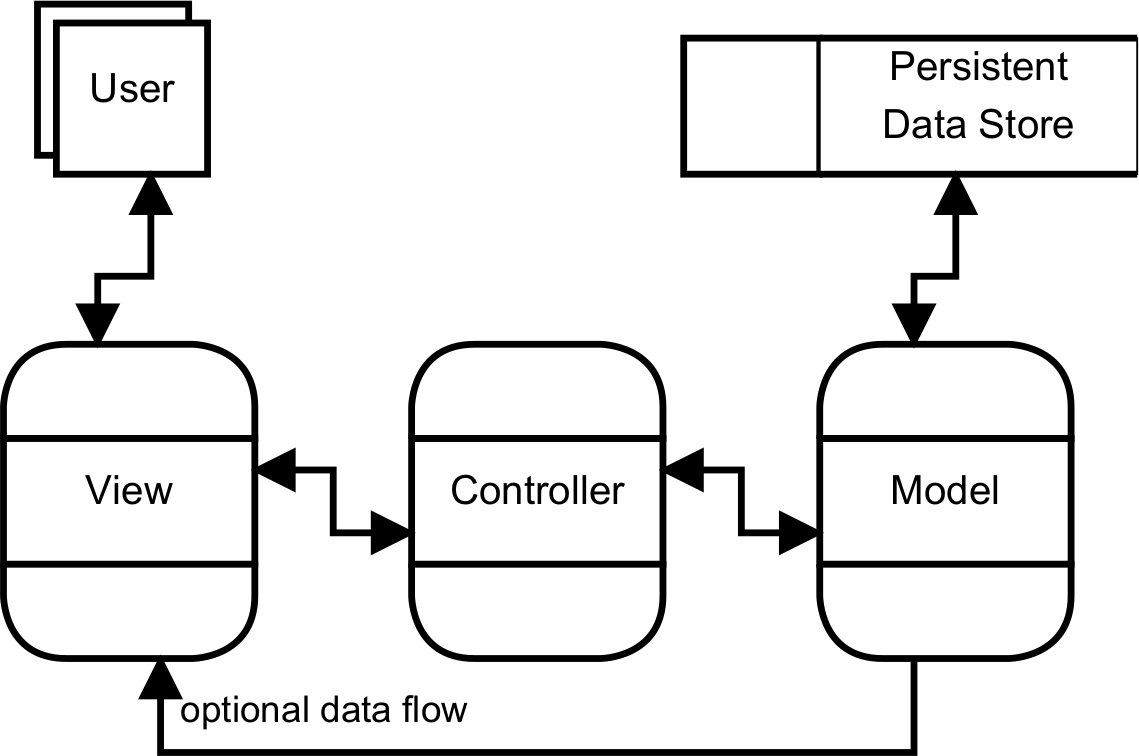
\includegraphics[width=.59\linewidth]{../img/mvc.png}}
    \normalcolor\vspace{-0.2em}\caption{Model-View-Controller aus \cite[Seite 177]{voorhees2020guide}}
\end{figure}

In Symfony heißen die Komponenten entsprechend \emph{View}, \emph{Controller} und Modell teilt sich auf in \emph{Repository} für Datenbankzugriffe sowie \emph{Service} für die Bereitstellung einer gewissen Funktionalität. \emph{Utility} ist für sonstige Klassen vorgesehen und \emph{Command} definiert Kommandozeilenbefehle außerhalb der MVC-Architektur. 

\newpara{Dependency Injection}

Das Ziel des Entwurfmusters Dependency Injection ist es die Instanziierung von Klassen einer zentralen Komponente zu überlassen, damit diese nicht von Änderungen untereinander abhängig sind und somit die Orthogonalität des Softwaresystem erhöht wird. Für eine ausführlichere Erklärung siehe \cite{seemann2019dependency}. In Symfony heißt die zentrale Komponente Container. Sie erkennt automatisch Klassen und stellt diese ohne notwendige Instanziierung in den Konstruktoren anderer Klassen zur Verfügung.

Das ermöglicht die Verwendung eines Services durch einen anderen zum Beispiel sehr einfach so:

\begin{Code}
class UmsteigerService {

    public function __construct(
        private readonly DataService $dataService
    ) {}

    public function searchAllUmsteigerVertical (
        string $system, $function = null): array {

        foreach ($this->dataService->getVersions($system) as $version) {
        // ...
\end{Code}

\newpara{Symfony-Komponenten}

Das \bfarmer-Projekt verwendet folgende Komponenten des Symfony-Frameworks:

\begin{itemize}
\item Console Commands \cite{symfony-command}\newline Zum Erstellen von Kommandozeilenbefehlen.
\item HttpFoundation Component \cite{symfony-http}\newline Für HTTP Request, Response, sowie Streaming. 
\item HTTP Client \cite{symfony-client}\newline Um Downloads zu starten. 
\item Filesystem Component \cite{symfony-file} \newline Für Dateioperationen. 
\item UID Component \cite{symfony-uuid} \newline Zum Generieren von UUIDs = URIs in den ConceptMaps. 
\item Controller \cite{symfony-controller} \newline Für Routing. 
\item Databases and the Doctrine ORM \cite{symfony-db} \newline Um Datenbankoperationen auszuführen.
\item Templates \cite{symfony-templates} und Twig Template Engine \cite{twig} \newline Für das Rendern von Webseiten.
\item Serializer Component \cite{symfony-serializer} \newline Zur Konvertierung von Daten. 
\end{itemize}

\begin{figure}[H]
    \centering
    \setlength{\fboxsep}{10pt}\color{black!20}\fbox{
    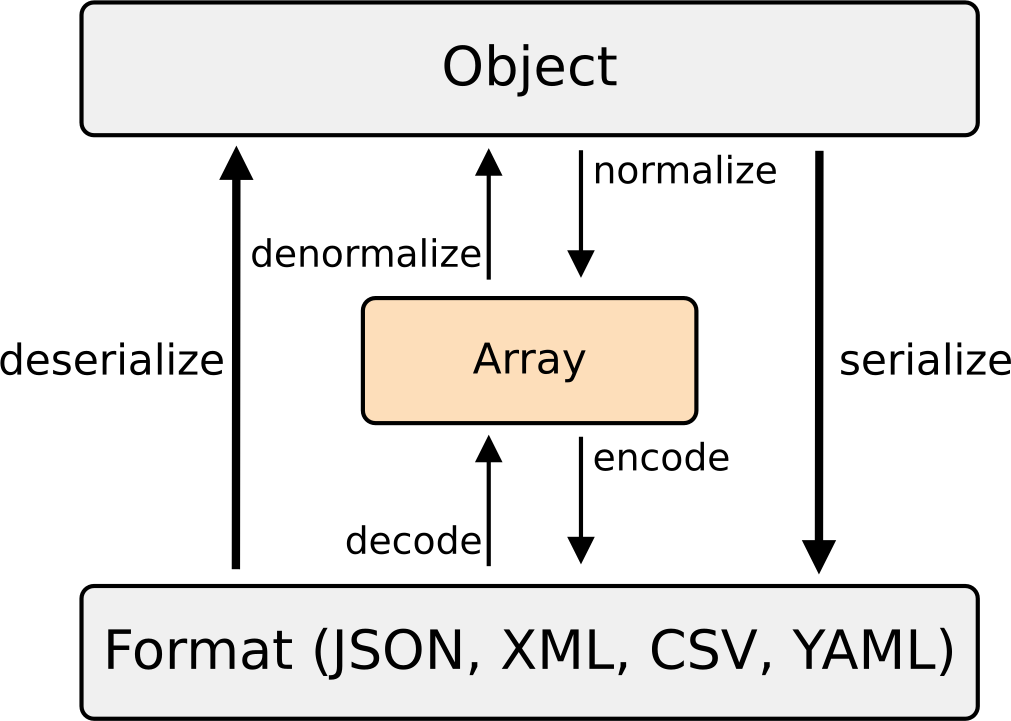
\includegraphics[width=.6\linewidth]{../img/serializer_workflow.png}}
    \normalcolor\caption{Schematische Darstellung der Serializer-Komponente \cite{symfony-serializer}}
\end{figure}

\vspace{-1.1em}

Serializer ist die wichtigste Symfony-Komponte im \bfarmer-Projekt. Sie dient zum: 

\begin{itemize}
\item Lesen der CSV-Dateien, in der die BfArM-Daten strukturiert sind.
\item Schreiben der ConceptMaps in XML oder JSON. Für eine nähere Erklärung der Datei-Formate siehe \cite[Seite 133ff]{bonnefoy2024definitive}.
\item Konfigurieren der ICD-10-GM und OPS Versionen in XML-Dateien.
\item Generieren von MySQL Insert-Statements mit einem eigenem Encoder.
\end{itemize}

\newpara{Anmerkung zu PHP}

Die Programmiersprache PHP hat unter Software-Entwicklern einen schlechten Ruf, obwohl --oder vielleicht auch weil-- sie von circa 75\% aller Webseiten verwendet wird laut \cite{w3techs}. In \cite{janssenscan} wird allerdings diskutiert, dass nicht das Verwenden einer bestimmter Programmiersprache gute Entwickler kennzeichnet, sonder das Verständnis über Programmierparadigmen, die leichter zu erlernen sind, je mehr Erfahrung mit verschiedenen Programmiersprachen gewonnen wurde. Das \bfarmer-Projekt ist bewusst möglichst modular, sowie unter Verwendung von möglichst vielen, weit verbreiteten Tools, Frameworks und Standardverfahren entwickelt, um auch die Übersetzung in eine andere Programmiersprache einfacher zu gestalten. 

\newpage

\section{Aufbau des \bfarmer-Projekts}

\subsection{Views}

\begin{itemize}
\item \texttt{base} \newline Grundvorlage für alle Seiten, also zum Beispiel \texttt{<head>} mit Imports für Stylesheets, Javascript und \texttt{<body>} mit den Inhalten.
\item \texttt{index} \newline Die Hauptseite der \bfarmer-Applikation. 
\item \texttt{codes} \newline Seite, welche alle Kodes einer Version anzeigt, inklusive Suchfunktion. 
\item \texttt{conceptmap} \newline Formular, um versionsübergreifende ConceptMaps zu generieren. Es kann eingestellt werden: Datei-Format, FHIR Release, Zielversion, ob Äquivalenzen ignoriert werden sollen.
\item \texttt{modal} \newline Format für das Modal, in dem zum Beispiel Ergebnisse der Umsteiger-Suche ausgehend von einem Kode angezeigt werden. Ein Modal ist wie ein Popup -- außer dass kein neues Fenster geöffnet wird. 
\item \texttt{umsteiger} \newline Übersicht über alle Umsteiger-Einträge; angezeigt jeweils zwischen zwei Versionen. Außerdem kann eine ConceptMap zwischen den beiden Versionen generiert werden. 
\item \texttt{umsteiger\_icons} \newline API-Schnittstelle, um eine Legende der Überleitung-Icons zu laden. 
\item \texttt{umsteiger\_search} \newline Seite, die es erlaubt nach Umsteigern für einen Kode zu suchen. 
\item \texttt{umsteiger\_search\_recursion}, \texttt{umsteiger\_search\_result}, \texttt{search\_code} \newline Dienen zur rekursiven Anzeige der Umsteiger-Suchergebnisse.
\end{itemize}

\subsection{Utility}

\begin{itemize}
\item \texttt{Constants} \newline Enthält globale Konstanten und statische Funktionen, um zum Beispiel eindeutige Namen für die SQL-Tabellen zu generieren. 
\item \texttt{SqlInsertEncoder} \newline Fügt mehrere Datensätze zu einem INSERT-Statements zusammen für die Integration. Dadurch werden die Daten wesentlich schneller in die Datenbank eingelesen, siehe \cite{mysql-insert}.
\item \texttt{TwigExtension} \newline Erweiterung der Twig Template Engine.
\end{itemize}

\subsection{Repositories}

\begin{itemize}
\item \texttt{BfarmRepository} \newline Dient zum Lesen und Schreiben der BfArM-Daten.
\item \texttt{ConfigRepository} \newline Speichert Informationen für den \bfarmer-Kommandozeilenbefehl. 
\item \texttt{DatabaseRepository} \newline Parent-Klasse der Repositories, um die Verbindung zur Datenbank aufzubauen. Stellt außerdem einen Wrapper für Operationen zur Verfügung, der SQL-Fehler loggt. 
\end{itemize}

\subsection{Controllers}

\begin{comment}
\begin{itemize}
\item \texttt{AdminController} \newline Lädt die Datenbank-GUI von \cite{adminer}.
\item \texttt{CodesController} \newline b
\item \texttt{ConceptMapController} \newline c
\item \texttt{DimdiController} \newline d
\item \texttt{IndexController} \newline e
\item \texttt{UmsteigerController} \newline g
\item \texttt{UmsteigerSearchController} \newline h
\end{itemize}
\end{comment}

\begin{itemize}
\item \texttt{AdminController} \newline Lädt die Datenbank-GUI von \cite{adminer}.
\item \texttt{CodesController}, \texttt{ConceptMapController}, \texttt{IndexController}, \newline
\texttt{UmsteigerController}, \texttt{UmsteigerSearchController}
\newline Reagieren auf Requests an die zugehörigen Views / API-Schnittstellen und generieren entsprechend Responses. Die Routes sind über Annotationen definiert. 
\item \texttt{DimdiController} \newline Stellt eine API-Schnittstelle für die externen Kode-Links der älteren ICD-10-GM und OPS Versionen zur Verfügung, siehe Abschnitt \ref{externe-kode-links}.
\end{itemize}

\subsection{Services}

\begin{itemize}
\item \texttt{ClientService} \newline Lädt Dateien und Inhalte von URLs herunter.
\item \texttt{ConceptMapService} \newline Enthält die Funktionen zum Schreiben der ConceptMap, siehe Abschnitt \ref{write-conceptmap}.
\item \texttt{DataService} \newline Liest Informationen über die ICD-10-GM / OPS Versionen aus den XML-Dateien. 
\item \texttt{SetupService} \newline Implementation des Datenintegrationsprozess. 
\item \texttt{UmsteigerService} \newline Implementation der horizontalen und vertikalen Umsteiger-Suche.
\end{itemize}

\subsection{Commands}

\begin{itemize}
\item \texttt{BfarmerCommand} \newline Kommandozeilenbefehle für die Datenintegration, siehe Abschnitt \ref{bfarm-cmd}.
\item \texttt{TestCommand} \newline Startet Tests, wie zum Beispiel den Vergleich zwischen den Ergebnissen aus der horizontalen und vertikalen Umsteiger-Suche. 
\end{itemize}

\subsection{Beispielanwendung}

Es gibt außerdem jeweils View, Repository,  Controller, Service und Command für die Beispielanwendung virtuelle Patientendatenbank, siehe Abschnitt \ref{virtpat} im nächsten Kapitel. 

\section{Backend}

\subsection{Setup-XML}

Die Versionen von ICD-10-GM und OPS, sowie die Abweichungen zwischen den Versionen sind in den XML-Dateien \texttt{files/icd10gm.xml} und \texttt{files/ops.xml} konfiguriert. Hier ein Auszug aus letzterer:

\begin{Code}
<?xml version="1.0" encoding="UTF-8"?>
<ops_setup>
    <ops>
        <year>2024</year>
        <url>https://multimedia.gsb.bund.de/BfArM/downloads/klassifikationen/ops/
            version2024/ops2024syst-ueberl.zip</url>
    </ops>
    <ops>
        <year>2023</year>
        <url>https://multimedia.gsb.bund.de/BfArM/downloads/klassifikationen/ops/
            version2023/ops2023syst-ueberl.zip</url>
    </ops>
<!-- ... -->
\end{Code}

Im Idealfall muss nur die Version und der Download-Link angegeben werden. 

%\newpage

\subsection{Kommandozeilenbefehle}
\label{bfarm-cmd}

Das Verarbeitung der Einträge in der XML-Konfiguration wird mit einem Kommandozeilenbefehl gestartet, der im Hauptverzeichnis des Projekts ausgeführt wird:

\begin{Code}
bin/console bfarmer --setup
\end{Code}

Dadurch wird pro Version der Datenintegrationsprozesses aus Abbildung \ref{bfarm-data-int} angestoßen. Für erfolgreiche integrierte Versionen wird ein Eintrag in der CONFIG-Tabelle erstellt, damit diese beim nächsten Aufruf übersprungen werden. Es gibt Optionen:

\begin{Code}
--icd10gm -i | Nur für ICD-10-GM ausführen.
--ops     -o | Nur für OPS ausführen.
--keep    -k | Die heruntergeladene Datei nicht löschen. 
\end{Code}

Folgender Befehl speichert zu jedem Kode, ob er Umsteiger hat: true/false. Ebenfalls mit Eintrag in der CONFIG-Tabelle, sowie den Optionen -i/-o. 

\begin{Code}
bin/console bfarmer --umsteiger
\end{Code}

Nach Erweiterung der XML-Datei um eine neue Version müssen also nur die zwei Befehle ausgeführt werden, um diese in die \bfarmer-Applikation aufzunehmen. 

\subsection{Datenbank}

Für die Datenbank wird MySQL \cite{mysql} als DB Management System verwendet und für den Verbindungsaufbau \cite{doctrine}. Nach aktuellen Entwicklungsstand laufen alle DB-Operationen über SQL-Befehle in MySQL, was zwar die Abstraktion der Datenbank verhindert, aber die Portabilität des \bfarmer-Projekt erhöht. 

Das BfArM schlägt folgende Tabellen in Microsoft-Access-Syntax vor, um die Kodes- und Umsteiger-Dateien zu importieren, zum Beispiel für ICD-10-GM 2024:

\begin{Code}
CREATE TABLE ICD10V2024 (
     Code2024   Text(7)    CONSTRAINT Code2024X PRIMARY KEY,
     Titel2024  Text(255)  
);

CREATE TABLE UMSTEIGER (
     Code2023       Text(7) CONSTRAINT UICD2023  REFERENCES ICD10V2023,
     Code2024       Text(7) CONSTRAINT UICD2024  REFERENCES ICD10V2024,
     Auto2023_2024  Text(1),
     Auto2024_2023  Text(1)
);
\end{Code}

%\newpage 

Stattdessen werden die Tabellen in \bfarmer so angelegt:

\begin{Code}
CREATE TABLE `ICD10GM_2024` (
  `code` varchar(7) NOT NULL,
  `name` varchar(255) DEFAULT NULL,
  `umst` tinyint(1) DEFAULT NULL,
  PRIMARY KEY (`code`)
) ENGINE=InnoDB DEFAULT CHARSET=utf8mb4 COLLATE=utf8mb4_unicode_ci;

CREATE TABLE `UMSTEIGER_ICD10GM_2024_2023` (
  `old` varchar(7) NOT NULL,
  `new` varchar(7) NOT NULL,
  `auto` varchar(1) DEFAULT NULL,
  `auto_r` varchar(1) DEFAULT NULL,
  PRIMARY KEY (`new`,`old`)
) ENGINE=InnoDB DEFAULT CHARSET=utf8mb4 COLLATE=utf8mb4_unicode_ci;
\end{Code}

Die Spaltennamen sind pro Tabellentyp gleich, was das Lesen vereinfacht. Hingegen sind die Tabellenname eindeutig pro Kodiersystem und Version. Der Key für die Umsteiger ist umgedreht, weil normalerweise die neueren Versionen links angezeigt werden. Außerdem gibt es Gründe Foreign Key Constraints zu vermeiden, siehe \cite{fkey-constraints}.

\section{Frontend}

Das Frontend basiert auf den Standardtechnologien HTML \cite{html}, zur Strukturierung der Inhalte auf den Seiten, CSS \cite{css}, für Layout und Styling der Inhalte und JavaScript \cite{javascript} für die Client-seitige, interaktive Veränderung von Inhalten. Beispielsweise wird das Ergebnis der horizontale Suche für M21.6 der ICD-10-GM 2013 so dargestellt:

\begin{figure}[H]
    \centering
    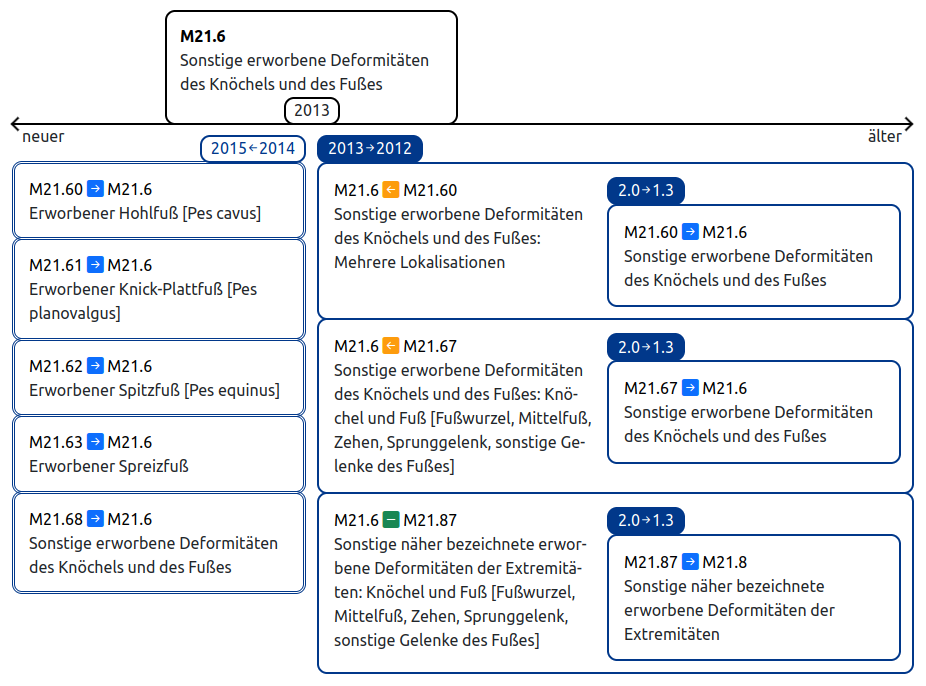
\includegraphics[width=\linewidth]{../img/umsteiger.png}
    \caption{Verwendung von HTML und CSS}
\end{figure}

Da das Ergebnis der horizontale Suche rekursiv aufgebaut ist, werden die Daten auch rekursiv gerendert. Die Variablen resultieren in verschiedene \texttt{<div>}-Blöcke, die jeweils mit einer eigenen CSS-Klasse gekennzeichnet sind. Eine Gruppe an Umsteigern wird also vertikal angeordnet unterhalb der Versionsnummern. Jeder Umsteiger-Eintrag erhält einen Rahmen und jeder Rekursionsschritt schiebt die anderen Ergebnisse nach außen. Dieses Layout basiert hauptsächlich auf Flexbox, siehe \cite{flexbox-csstricks}. 

Außerdem verwendet werden:

\begin{itemize}
\item SASS/SCSS \cite{sass}, um das Schreiben von CSS zu vereinfachen. Aus der Skriptsprache SCSS wird CSS kompiliert wird. Merkmale sind beispielsweise ein geschachtelte Syntax, welche die Verwendung von CSS-Selektoren vereinfacht, sowie Variablen und Funktionen, zum Beispiel für die Berechnung von Pixelbreiten. 
\item Popper.js \cite{popperjs} für Tooltips.
\item Bootstrap \cite{bootstrap} für das Basis-Layout, Header-Banner, Navigation-Tabs, Modals und Icons. 
\item jQuery \cite{jquery}, um beispielsweise Modal-Content per AJAX zu füllen, siehe den nächsten Abschnitt \ref{ajax-sec}.
\end{itemize}

Eingebunden werden diese Tools über Webpack \cite{webpack}, einem JavaScript-Modul-Packer, der wiederum auf der JavaScript-Laufzeitumgebung Node.js \cite{nodejs} und dem zugehörigen JavaScript-Paketmanager NPM \cite{npm} aufbaut. 

\begin{comment}


, sowie JavaScript , für interaktive Bedienungselemente. 

\subsection{Webpack / Node.js}

Webpack , NPM \cite{npm}, Node.js 

webpack is a static module bundler for modern JavaScript applications


\subsection{Bootstrap}

Bootstrap

Layout, Nav-Tabs, Modal, Icons

\subsection{SCSS}

\subsection{Tooltips}
\end{comment}

\section{AJAX}
\label{ajax-sec}

Der Begriff AJAX, \emph{Asynchronous JavaScript and XML}, wurde erstmals in \cite{garrett2005ajax} geprägt, beschreibt aber damals schon verbreitete Ansätze zur Interaktion mit Webseiten.

\begin{figure}[H]
    \centering
    \setlength{\fboxsep}{5pt}\color{black!20}\fbox{
    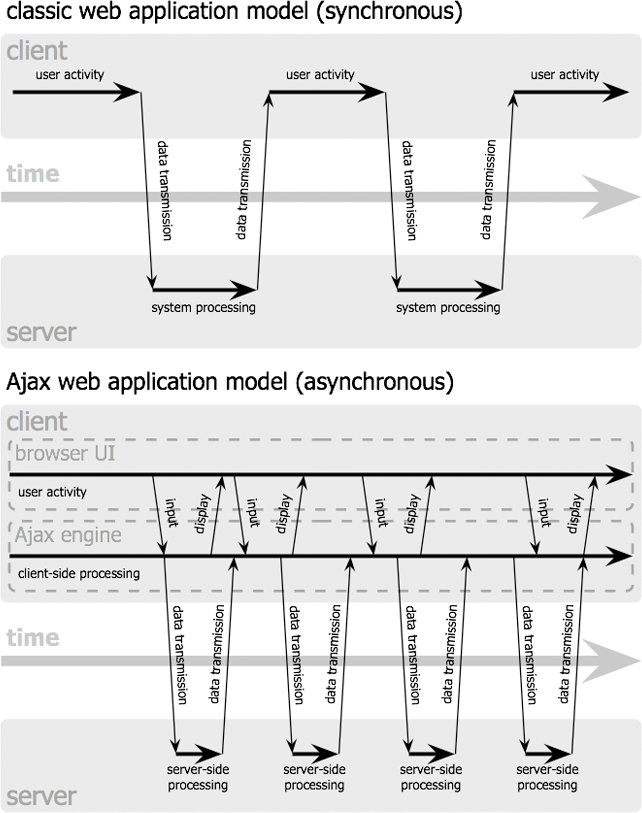
\includegraphics[width=.65\linewidth]{../img/ajax.png}}
    \normalcolor\vspace{-0.5em}\caption{Klassisches und AJAX Web-Applikations-Modell nach \cite{garrett2005ajax}.}
\end{figure}

Statt dass wie gewöhnlich eine Interaktion das Laden einer ganzen Seite auslöst, erlaubt die AJAX-Engine durch Versenden von Requests, was als JavaScript Client-seitig passiert, das Verändern einzelner Teile einer Seite. Anders als der Name andeutet muss es sich dabei aber nicht um XML-Daten handeln, sondern AJAX funktioniert über jede Art von HTTP-Request. 

In \bfarmer wird AJAX verwendet, um Bootstrap-Modals nach Klick auf ein Umsteiger-Icon mit Inhalt zu füllen. Dazu mehr im Abschnitt \ref{virtpat}. 

\subsection{Externe Links zu den BfArM/DIMDI Kode-Seiten}
\label{externe-kode-links}

Außerdem dient AJAX dazu, externe Links auf die BfArM- beziehungsweise DIMDI-Seiten zu öffnen, welche mehr Information für Kodes anzeigen. Diese Links werden per Klick auf jeden Kode auf den \bfarmer-Seiten bereitgestellt.

Dabei besteht die Schwierigkeit besteht darin, dass die URLs für die Kode-Informationen auf den BfArM- und DIMDI-Seiten nicht einfach nur durch Kodiersystem, Version und Kode besteht. Sondern es muss zusätzlich noch die Kode-Gruppe ermittelt werden. Das ist nicht trivial, weil die Gruppe nicht über den Kode bestimmt werden kann. 

Beispiel: \texttt{https://www.dimdi.de/static/de/klassifikationen/icd/icd-10-gm/\newline kode-suche/htmlgm2013/block-m20-m25.htm\#M21} -- Die Gruppe ist m20-m25. Manchmal enthält die Gruppe aber gar nicht die Zeichen des Kodes.

Die BfArM- und DIMDI-Server stellen zwar JavaScript-Dateien zur Verfügung, die eine Funktion zum Bestimmen der Gruppe für einen gegebenen Kode enthält, allerdings heißt diese Funktion immer gleich und jede Datei enthält immer nur die Gruppen für eine Version. Das heißt es ist nicht möglich, wenn auf den \bfarmer-Seiten zum Beispiel im Ergebnis der Umsteiger-Suche mehrere Kodes von mehreren Versionen angezeigt werden, alle diese Dateien zu laden, um die Gruppen zu bestimmen, weil die Funktionen in den Dateien sich gegenseitig überschreiben und so über diese Vorgehensweise immer nur pro Seite die Gruppen \emph{einer} Version ermittelt werden könnten. 

Stattdessen muss beim Klick auf einen Kode die jeweils passende Datei der Version des Kodes per AJAX geladen und ausgeführt werden. Die Dateien befinden sich ab 2015 auf der BfArM-Seite und vorher auf dem DIMDI-Seite, das heißt hier muss außerdem noch eine Differenzierung passieren. Weiterhin kommt erschwerend hinzu, dass für ICD-10-GM Versionen älter als 2008 und OPS Versionen älter als 2009 die DIMDI-Seiten die JavaScript-Funktionen gar nicht als einzelne Dateien anbieten, sondern diese ist innerhalb von HTML-Seiten eingebettet. Um wiederum dieses Problem zu lösen, gibt es eine zusätzliche API-Schnittstelle im \bfarmer-Projekt, welche die HTML-Seiten dieser älteren Versionen lädt, die JavaScript-Funktionalität extrahiert und zurückgibt. Der AJAX-Aufruf geht dann also erst an die eigene Schnittstelle.

\begin{comment}
Die Vorgehensweise ist also wie folgt:

\begin{enumerate}
\item Kode der ICD-GM-10 und OPS Versionen 2015 oder neuer: Lade die JavaScript-Datei für die passende Version vom BfArM-Server per AJAX und führe das Skript aus, um die Kode-Gruppe zu ermitteln. Dann benutze diese um die URL zu bauen und öffne die BfArM-Kode-Seite. 
\item Kode der ICD-GM-10 2014 bis 2009 oder OPS 2014 bis 2010: Wie oben, aber über die DIMDI-Seite. 
\end{enumerate}
\end{comment}

Weil das Öffnen von Links nach einem AJAX-Aufruf von Browsern als Popup wahrgenommen und meist blockiert wird, muss das Fenster oder der Tab in dem die BfArM- oder DIMDI-Seite geladen werden soll, schon vor Ausführen des AJAX-Codes geöffnet werden. 


% mit einer neuen Struktur aufzubauen, die über das gewöhnliche Laden einer ganzen Seite pro Interaktion hinausgeht. Stattdessen 

\begin{comment}
API-Schnittstellen

Modal

BfArM/Dimdi Links -- Neuer Tab muss geöffnet werden bevor Skripte ausgeführt werden. \label{externe-kode-links}

\subsection{Anonyme Funktionen}

Callback

Zum Schreiben der ConceptMap

Data-Preprocessing

InsertEncoder
\end{comment}

